%\section{Applying cuts to the same flavour channel}
\section{First view}

A common practice in SUSY dilepton analyses is to divide events into same flavour (SF) and different flavour (DF) varieties. SF thus includes events with pairs of only electrons or only muons in their final states, and DF refers to the events that decay into an electron-muon pair. In this analysis this convention will be followed.

The preliminary cuts on the pair of electrons were $\mathbf{p}_{\text{T},e_1}>$ 25 GeV and $\mathbf{p}_{\text{T},e_2}>$ 20 GeV, where $e_1$ refers to the leading lepton with the largest momentum and $e_2$ to the second one.  For a muon pair the following requirements were imposed: leading muon $\mathbf{p}_{\text{T},\mu_1}>$ 25 GeV, second muon $\mathbf{p}_{\text{T},\mu_2}>$ 10 GeV, and the invariant mass $m_{\mu \mu}>$ 20 GeV. These cuts were motivated by the trigger efficiency for offline lepton candidates' identification (see Fig. \ref{fig:eltrig} and \ref{fig:mutrig} in the appendix \ref{app:triggers}).

First, histograms showing the entirety of the 2015 data, MC background and signal simulations were plotted. Fig. \ref{fig:SF_total_mll} shows the distribution of the \dileptonmass \, in the SF channel. The largest background contributions come from $Z$+jets, diboson, and $t\bar{t}$ processes. 
The pronounced peak in the SF dilepton invariant mass distribution is in the 80-100 GeV bin due to the contribution from the $Z$+jets component. This background can be suppressed by introducing $m_Z$-veto which cuts out all events within 10 GeV from the mass of the $Z$ boson (91.2 GeV). However, after this cut, the distribution will still retain events from the off mass-shell decays of the $Z$ boson. 

The histogram for DF channel (Fig. \ref{fig:DF_total_mll}) shows that there is a much smaller contribution from $Z$+jets component in this channel compared to the SF one. Thus $m_Z$ veto here can be avoided. The diboson and $t\bar{t}$ processes, however, prevail in this channel as well. 

\begin{figure}[!th]	   
	\begin{subfigure}[t]{0.5\textwidth}
		\subcaption{} 
		\label{fig:SF_total_mll}
        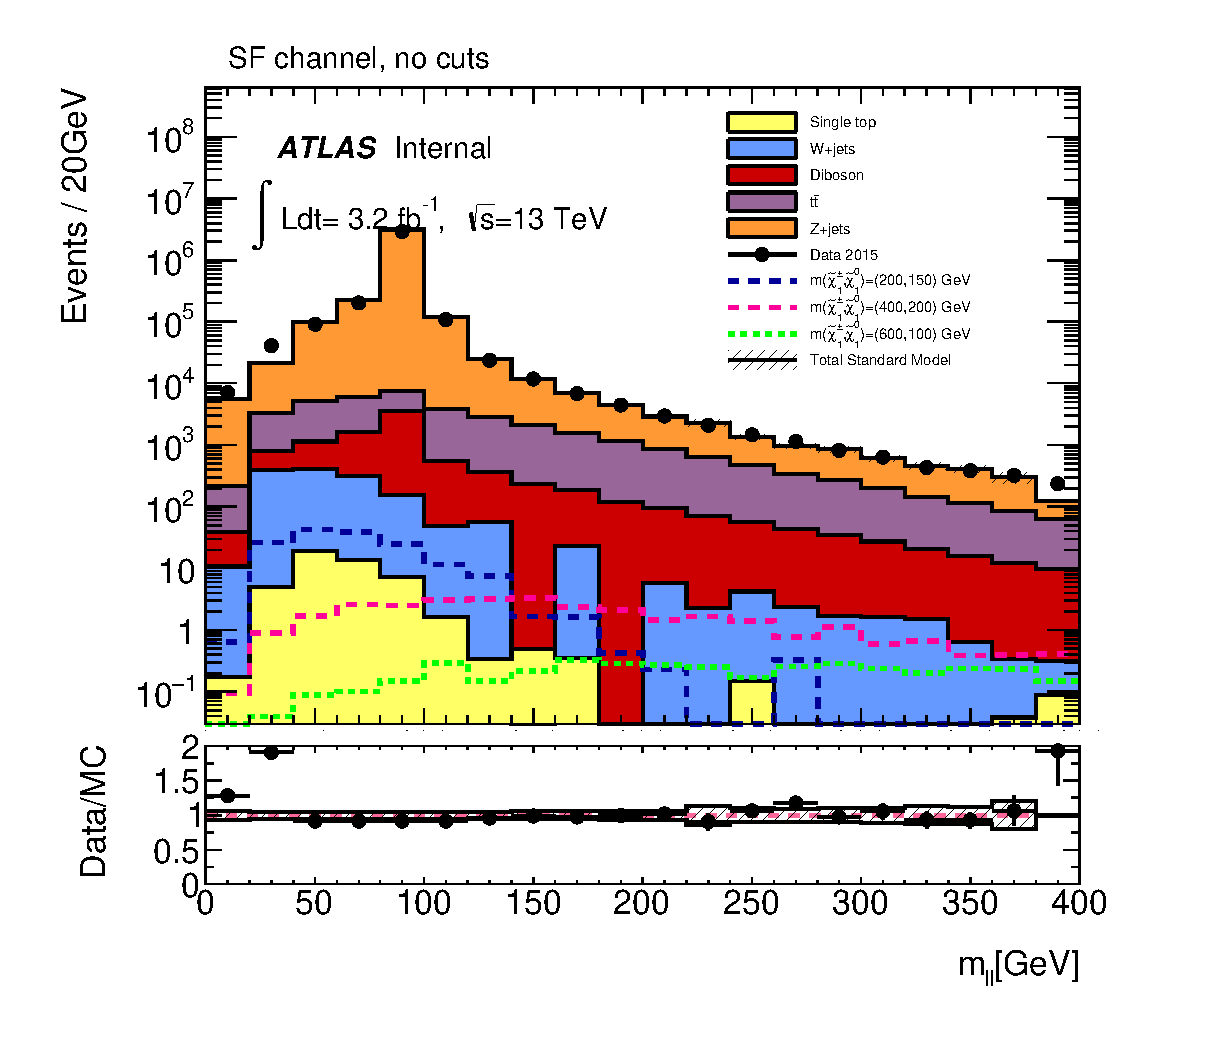
\includegraphics[scale=0.38]{Chap4/SF_DileptonMll_13TeV_total_signal} 
        \end{subfigure} 
     \begin{subfigure}[t]{0.5\textwidth}
     \subcaption{}
     	\label{fig:DF_total_mll}
        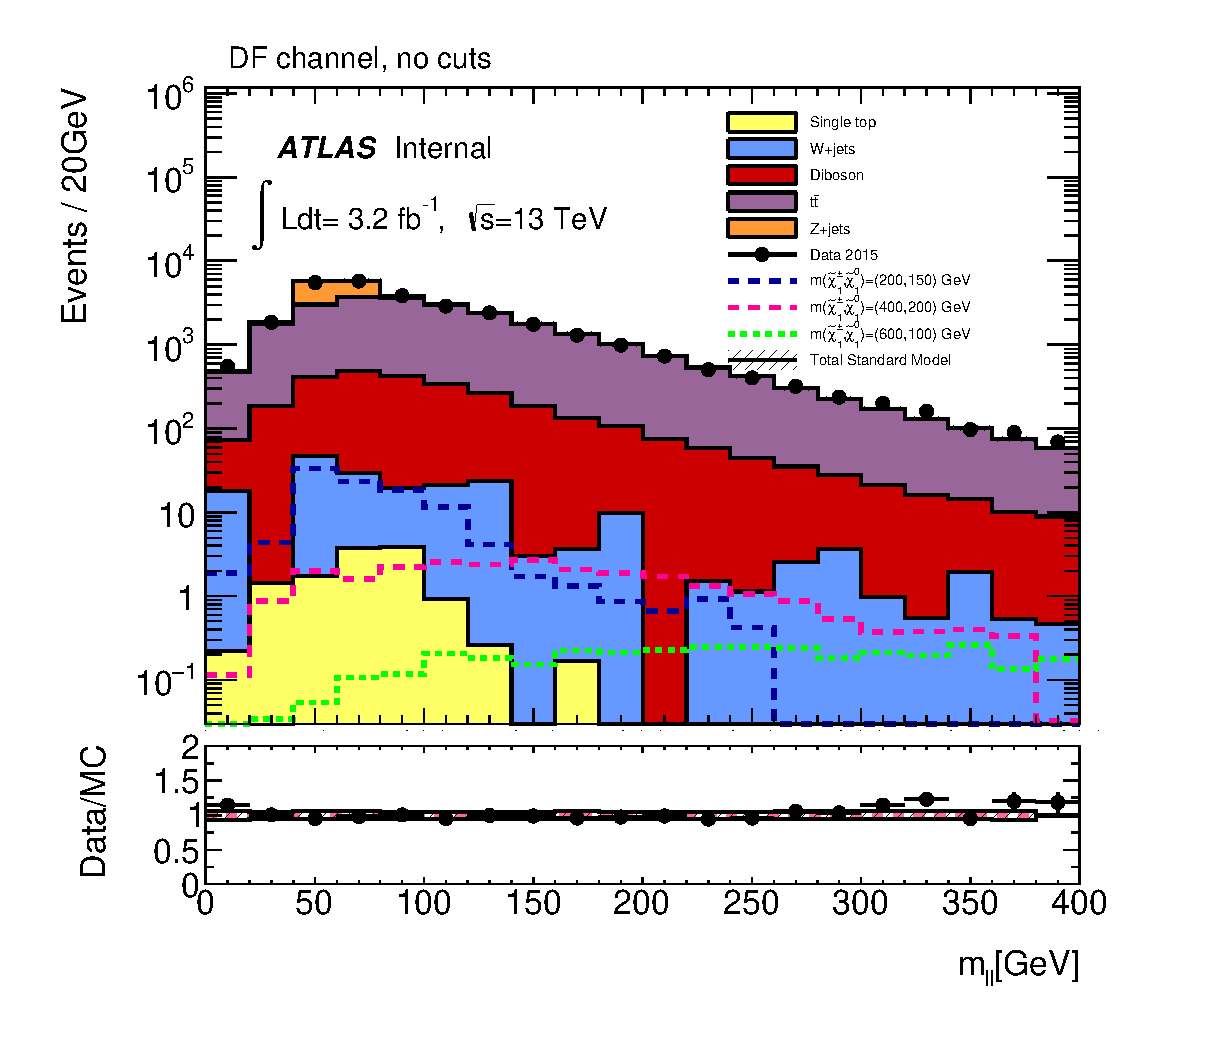
\includegraphics[scale=0.38]{Chap4/Emu_DileptonMll_13TeV_total_signal} 
        \end{subfigure}
        \begin{subfigure}[t]{0.5\textwidth}
		\subcaption{} 
		\label{fig:SF_total_mt2}
        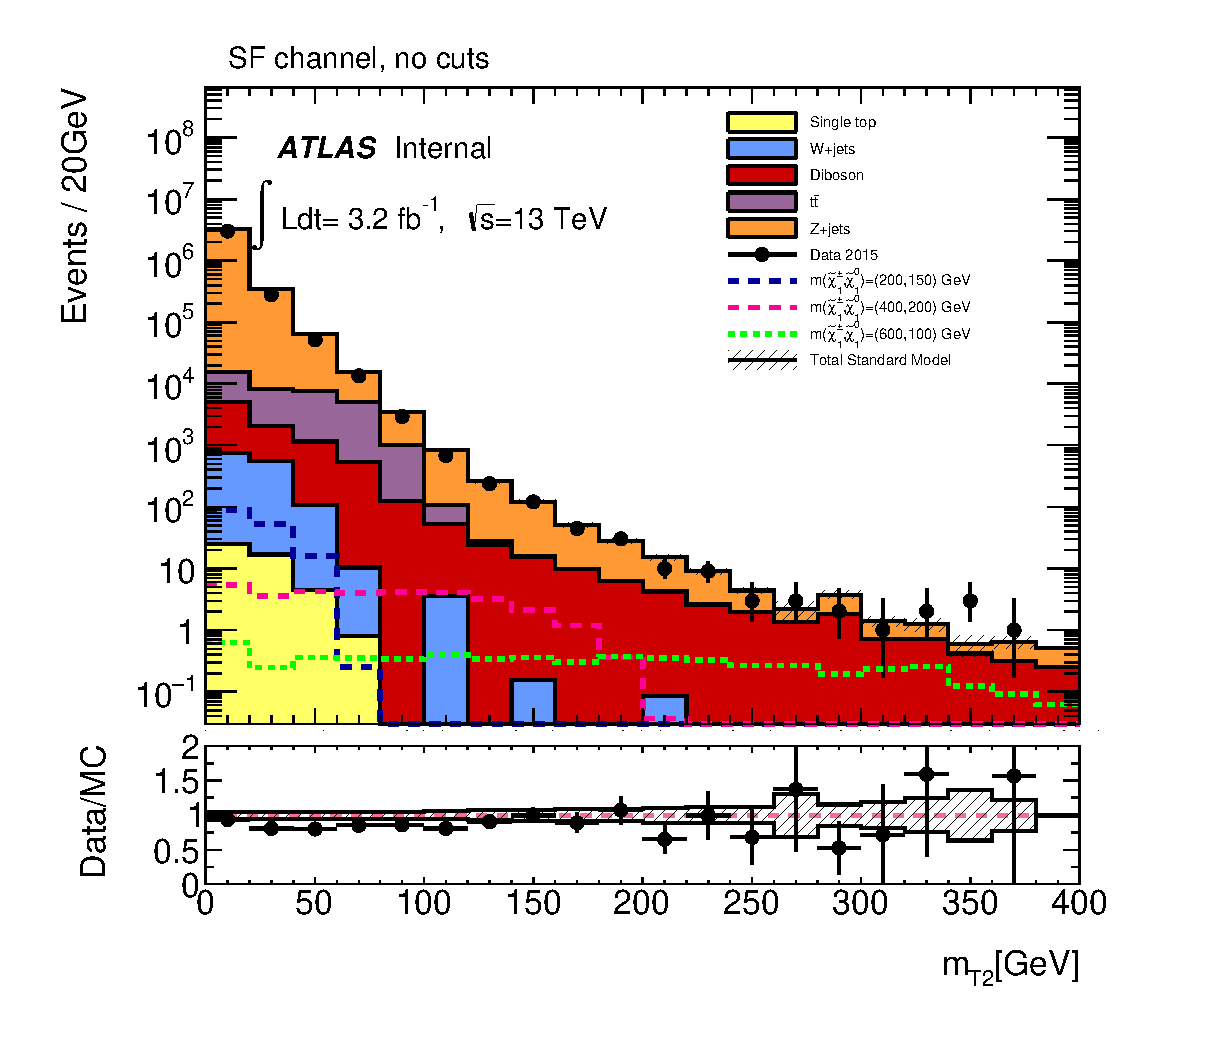
\includegraphics[scale=0.38]{Chap4/SF_DileptonMt2_13TeV_total_signal} 
        \end{subfigure} 
     \begin{subfigure}[t]{0.5\textwidth}
     \subcaption{}
     	\label{fig:DF_total_mt2}
        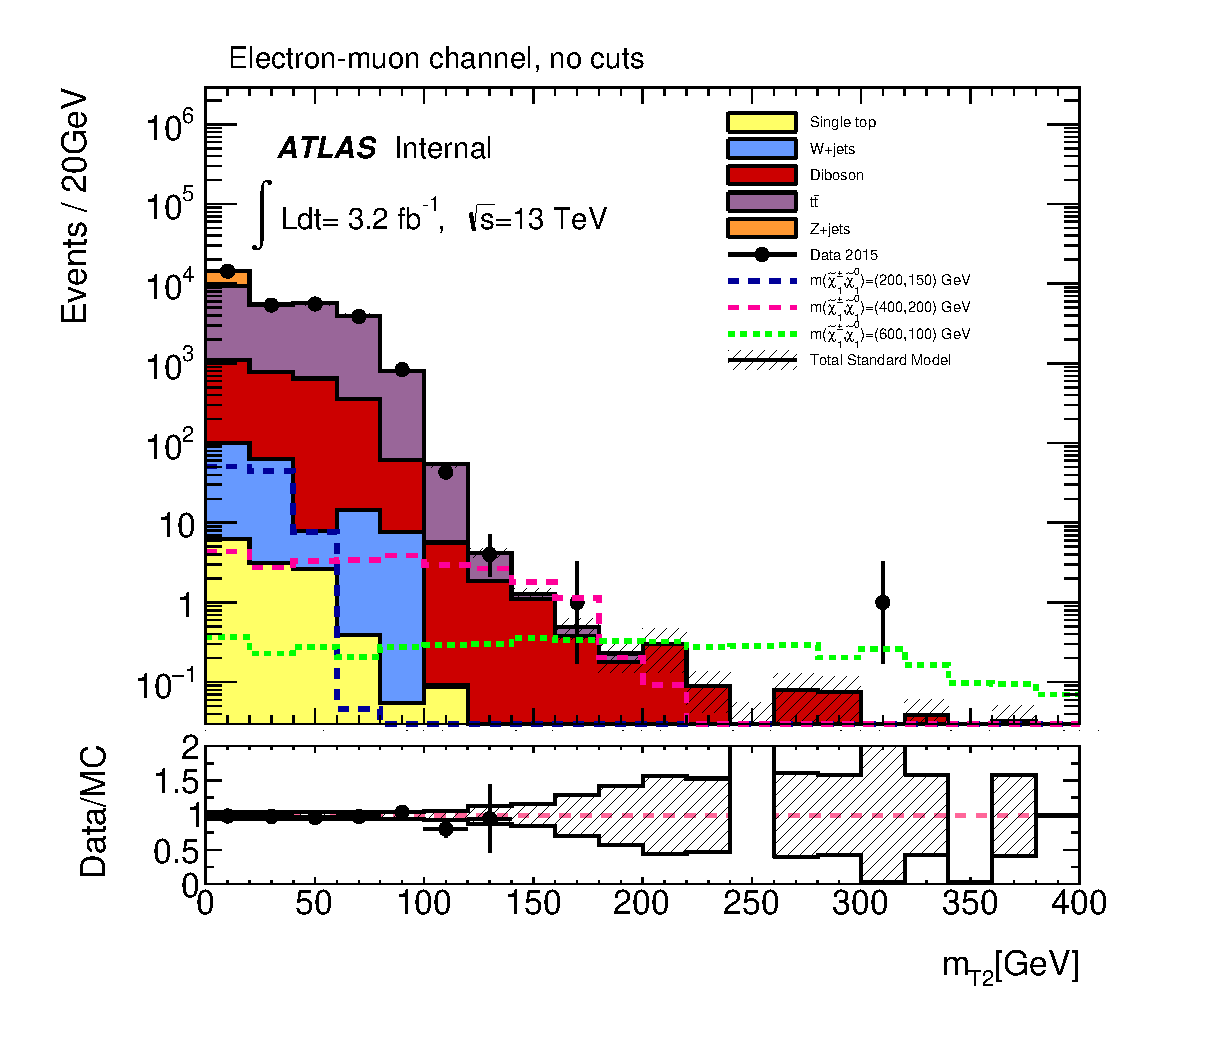
\includegraphics[scale=0.38]{Chap4/Emu_DileptonMt2_13TeV_total_signal} 
        \end{subfigure}
\caption{Distribution of $m_{\ell \ell}$ and \mttwo \, variables for SF and DF channels for all events.}	
        \label{fig:Elmu_total_histos}
\end{figure}

The dotted lines are the shapes of signal distributions and they are in accordance with the mass of the chargino pair. The blue line represents 200-150 mass splitting, so its events are concentrated in the lower mass regions. The pink and green lines represent 400-200 and 600-100 signals respectively, and also are distributed according to this logic. Overall, there is a good agreement between MC background simulations and the 2015 data. 

\newpage
\section{Applying cuts}
\subparagraph{Veto on all jets.}

As was mentioned in the previous section the the following veto was imposed on all the signal regions in SF channel:
\begin{equation*}
|m_{\ell \ell} - m_Z| > 10 \text{ GeV (with } m_Z = 91.2 \text{ GeV}) 
\end{equation*}
This veto was common for all further analyses in the SF channel, however it was not used at all for the DF channel.
The next step was to veto all the jets to reduce $t\bar{t}$ contribution. The result of this combination of vetoes can be seen in Fig. \ref{fig:0jets_mz}. As expected the \mttwo \, distribution is dependent on the mass splitting and is better for the 400-200 and 600-100 signals. At this point it is possible to calculate sensitivity values by placing cuts on \mttwo \, and the results can be seen in Tab. \ref{tab:SF_score}. No events from the 200-150 signal model passed the cuts, therefore it is omitted from the table. The best result for SF channel was the projected significance of 3.62 at 19.2 fb\textsuperscript{-1}  with \mttwo$>100$ GeV cut. The same cut for DF channel lead to 5.15 of significance at 19.2 fb\textsuperscript{-1}. Significances for the 600-100 signal were not high in both channels, but were better for DF distributions, although not overwhelmingly so. 

\begin{figure}[h!]
\captionsetup{width=0.8\textwidth}	   
	\begin{subfigure}[t]{0.5\textwidth}
		\subcaption{$|m_{\ell \ell} - m_Z| > 10$ GeV, no jets} 
		\label{fig:SF_0jets_mz_mt2}
        \includegraphics[scale=0.38]{Nojetsmz/SF_DileptonMt2_13TeV_0jets_mz_signal} 
        \end{subfigure} 
     \begin{subfigure}[t]{0.5\textwidth}
		\subcaption{No jets} 
		\label{fig:DF_0jets_mz_mt2}
        \includegraphics[scale=0.38]{Nojetsmz/Emu_DileptonMt2_13TeV_0jets_mz_signal} 
        \end{subfigure}      
\caption{The \mttwo \, distributions for SF and DF channels, with cuts on $m_Z$ (only for SF events) and no jets.}	
        \label{fig:0jets_mz}
\end{figure}
\begin{table}[H]
\centering
\captionsetup{width=0.8\textwidth}
\begin{tabular}{|l|llllll}
\hline
Signal models     & \multicolumn{1}{l|}{400-200} & \multicolumn{1}{l|}{600-100} & \multicolumn{1}{l|}{400-200} & \multicolumn{1}{l|}{600-100} & \multicolumn{1}{l|}{400-200} & \multicolumn{1}{l|}{600-100} \\ \hline
\hspace{5mm} $\int L\, \mathrm{dt}$     & \multicolumn{2}{c|}{3.2 fb-1}                                                     & \multicolumn{2}{c|}{9.6 fb-1}                                                     & \multicolumn{2}{c|}{19.2 fb-1}                                                    \\ \hline 
 \mttwo \, cut [GeV]            & \multicolumn{6}{c|}{\textbf{SF channel}}                                                                                                                                                                                                                   \\ \hline
$>80$  & \multicolumn{1}{l|}{1.01}               & \multicolumn{1}{l|}{0.26}               & \multicolumn{1}{l|}{1.74}               & \multicolumn{1}{l|}{0.45}               & \multicolumn{1}{l|}{2.46}               & \multicolumn{1}{l|}{0.64}               \\ \hline
$>100$ & \multicolumn{1}{l|}{1.47}               & \multicolumn{1}{l|}{0.50}               & \multicolumn{1}{l|}{2.56}               & \multicolumn{1}{l|}{0.86}               & \multicolumn{1}{l|}{3.62}               & \multicolumn{1}{l|}{1.22}               \\ \hline
$>120$  & \multicolumn{1}{l|}{1.27}               & \multicolumn{1}{l|}{0.61}               & \multicolumn{1}{l|}{2.19}               & \multicolumn{1}{l|}{1.06}               & \multicolumn{1}{l|}{3.09}               & \multicolumn{1}{l|}{1.5}                \\ \hline
                  & \multicolumn{6}{c|}{\textbf{DF channel}}                                                                                                                                                                                                                  \\ \hline
$>80$   & \multicolumn{1}{l|}{1.12}               & \multicolumn{1}{l|}{0.31}               & \multicolumn{1}{l|}{1.95}               & \multicolumn{1}{l|}{0.54}               & \multicolumn{1}{l|}{2.76}               & \multicolumn{1}{l|}{0.76}               \\ \hline
$>100$   & \multicolumn{1}{l|}{2.10}               & \multicolumn{1}{l|}{0.75}               & \multicolumn{1}{l|}{3.64}               & \multicolumn{1}{l|}{1.30}               & \multicolumn{1}{l|}{5.15}               & \multicolumn{1}{l|}{1.83}               \\ \hline
$>120$    & \multicolumn{1}{l|}{2.10}               & \multicolumn{1}{l|}{1.07}               & \multicolumn{1}{l|}{3.65}               & \multicolumn{1}{l|}{1.86}               & \multicolumn{1}{l|}{5.16}               & \multicolumn{1}{l|}{2.63}               \\ \hline
\end{tabular}
\caption{Significance values ($S/\sqrt{B}$) for the SF and DF channel signal models with various cuts on \mttwo \, at increasing integrated luminosities. Cuts are placed on $m_Z$ (only for SF) and no jets are allowed.}
\label{tab:SF_score}
\end{table}

This cut follows previous ATLAS searches in dilepton channel, albeit those studies used signals with different chargino masses. 
%citation here!!!!


\subparagraph{Veto on $b$-tagged jets.}

Instead of vetoing all jets a different cut vetoing only $b$-tagged jets was made and the resulting histograms can be seen in Fig. \ref{fig:SF_0bjets_mz}. The $b$-jet veto is evidently less drastic and leads to both more background and signal events in the final distribution. However, to see whether this cut makes difference compared to the no-jets cut, the significances have to be calculated. The resulting values can be seen in Table \ref{tab:SF_score_0bjets}. Again, no events from the 200-150 signal model passed the cuts and this model was omitted.

The $b$-jet veto leads to a decrease in significance for SF channel compared to the same cuts with no-jets cut. However, for DF channel significance values are higher and at 19 \invfb they are 6.77 and 3.88 for the 400-200 and 600-100 signals respectively. This difference is due to the effect of the $Z$+jets background. It is suppressed better in the SF channel by cutting all jets. 

\begin{figure}[H]	   
	\begin{subfigure}[t]{0.5\textwidth}
		\subcaption{$|m_{\ell \ell} - m_Z| > 10$ GeV, no $b$-jets} 
		\label{fig:SF_0jets_mz_mt2}
        \includegraphics[scale=0.38]{Chap4/SF_DileptonMt2_13TeV_0bjets_mz_signal} 
        \end{subfigure} 
     \begin{subfigure}[t]{0.5\textwidth}
     \subcaption{No $b$-jets}
     	\label{fig:SF_0jets_mz_metrel}
        \includegraphics[scale=0.38]{Chap4/Emu_DileptonMt2_13TeV_0bjets_mz_signal} 
        \end{subfigure}
        \captionsetup{width=0.8\textwidth}
\caption{The \mttwo \, distributions for SF and DF channels, with cuts on $m_Z$ and no $b$-jets.}	
        \label{fig:SF_0bjets_mz}
\end{figure}
\begin{table}[H]
\centering
\captionsetup{width=0.8\textwidth}
\begin{tabular}{|l|llllll}
\hline
Signal models     & \multicolumn{1}{l|}{400-200} & \multicolumn{1}{l|}{600-100} & \multicolumn{1}{l|}{400-200} & \multicolumn{1}{l|}{600-100} & \multicolumn{1}{l|}{400-200} & \multicolumn{1}{l|}{600-100} \\ \hline
\hspace{5mm} $\int L\, \mathrm{dt}$     & \multicolumn{2}{c|}{3.2 fb-1}                                                     & \multicolumn{2}{c|}{9.6 fb-1}                                                     & \multicolumn{2}{c|}{19.2 fb-1}                                                    \\ \hline 
 \mttwo \, cut [GeV]            & \multicolumn{6}{c|}{\textbf{SF channel}}                                                                                                                                                                                                                   \\ \hline
$>80$  & \multicolumn{1}{l|}{0.48}               & \multicolumn{1}{l|}{0.14}               & \multicolumn{1}{l|}{0.84}               & \multicolumn{1}{l|}{0.25}               & \multicolumn{1}{l|}{1.19}               & \multicolumn{1}{l|}{0.35}               \\ \hline
$>100$ & \multicolumn{1}{l|}{0.63}               & \multicolumn{1}{l|}{0.24}               & \multicolumn{1}{l|}{1.09}               & \multicolumn{1}{l|}{0.41}               & \multicolumn{1}{l|}{1.54}               & \multicolumn{1}{l|}{0.59}               \\ \hline
$>120$  & \multicolumn{1}{l|}{0.65}               & \multicolumn{1}{l|}{0.34}               & \multicolumn{1}{l|}{1.12}               & \multicolumn{1}{l|}{0.60}               & \multicolumn{1}{l|}{1.58}               & \multicolumn{1}{l|}{0.84}                \\ \hline
                  & \multicolumn{6}{c|}{\textbf{DF channel}}                                                                                                                                                                                                                  \\ \hline
$>80$   & \multicolumn{1}{l|}{0.94}               & \multicolumn{1}{l|}{0.29}               & \multicolumn{1}{l|}{1.64}               & \multicolumn{1}{l|}{0.50}               & \multicolumn{1}{l|}{1.49}               & \multicolumn{1}{l|}{0.45}               \\ \hline
$>100$   & \multicolumn{1}{l|}{2.06}               & \multicolumn{1}{l|}{0.85}               & \multicolumn{1}{l|}{3.57}               & \multicolumn{1}{l|}{1.47}               & \multicolumn{1}{l|}{5.05}               & \multicolumn{1}{l|}{2.08}               \\ \hline
$>120$    & \multicolumn{1}{l|}{2.76}               & \multicolumn{1}{l|}{1.59}               & \multicolumn{1}{l|}{4.79}               & \multicolumn{1}{l|}{2.75}               & \multicolumn{1}{l|}{6.77}               & \multicolumn{1}{l|}{3.88}               \\ \hline
\end{tabular}
\caption{Significance values for the SF and DF channels with cuts on \mttwo \, at increasing integrated luminosities. Vetoes are placed on $m_Z$ (SF only) and $b$-jets. }
\label{tab:SF_score_0bjets}
\end{table}


